
\section{Derivatives of Radial Basis Functions}
\label{sec:rbf}

In this paper, we propose a new idea that is applicable to radial
basis functions (RBFs). Their strength is the ability to randomly
distribute points across complex physical domains, and have an
implementation that is independent of dimensionality. RBFs approximate
a function $f(\rvec)\subset \mathbb{R}^d$ sampled at a set of $N$
distinct point locations, $x_j$, by linearly combining translates of a
single radially symmetric function $\phi(r)$, where $r =
\|\rvec-\rvec_{j}\|$ denotes the Euclidean distance %(e.g., in 2-D
%$\sqrt{(x-x_j)^2+(y-y_j)^2}$) 
between $\rvec$, where the function is evaluated
and and $\rvec_j$,  where the RBF is centered. That is, the
interpolant is $s(\rvec) = \sum_{j=1}^{N} w_j
\phi_i(\|\rvec-\rvec_{j}\|)$. The weights $w_j$ are obtained by
inverting the system
\begin{equation}
\parray{lccr}{
\phi_{11} & \phi_{12} & \cdots & \phi_{1N} \\
\vdots & \ddots & \vdots & \vdots \\
\phi_{n1} & \phi_{n2} & \cdots & \phi_{NN} 
}
\parray{c}{ w_{1} \\ \vdots \\ w_{N} }
=
\parray{c}{ f(\rvec_1) \\ \vdots\\ f(\rvec_N) }. 
\label{eq:rbf}
\end{equation}
where $\phi_{ij} = \phi(\|\rvec_i-\rvec_j\|)$. 

The RBF differentiation matrix, $D_N$, is derived by applying the
desired analytic derivative operator $L$ to the RBF interpolant
$s(\rvec)$ above and evaluating it at the point locations. For very
large problems, this is a computationally expensive since the matrix
in (\ref{eq:rbf}) is full and inversion requires O$(N^3)$
operations. To alleviate the cost of this global approach (i.e., using
every node in the domain to calculate the derivative at a given node
$\rvec_i$), RBF-generated finite differences (RBFFD) have been
derived \cite{TAI1,TAI2,SDY02,WrFo06,FoL11,FLBWSC12}. RBFFD uses only
a local set of the $n_z-1$  (often nearest) points in a neighborhood of 
the point $\rvec_i$ to
approximate the derivative. In other words,
$Lf(\rvec_i)=\sum_{j=1}^{n_z}a_jf(\rvec_j)$. The differentiation
weights, $a_j$, are calculated by enforcing that this linear
combination should be exact for RBFs,
$\{\phi(\|\rvec-\rvec_{j}\|)\}_{j=1}^{n_z}$, centered at each of the
node locations $\{\rvec_j\}_{j=1}^{n_z}$ (classical finite-differences
(FD) would enforce that it be exact for polynomials instead.) Similar
to FD, as the stencil size $n_z$ increases so does the order of the
method.

For a total of $N$ points, there will be $N$ linear systems to solve,
each of size $n_z \times n_z$. Each linear solve produces a row of the
RBFFD differentiation matrix $A_{n_z}$, resulting in a $N \times N$
matrix with $n_zN$ nonzero entries. To evaluate the derivative at all
points in the domain, one multiplies the source vector $x$ by the 
derivative matrix $A$ to obtain the vector $y$ of derivative values, 
$$
  y = A x
$$
The computation of a single derivative has been reduced to a SpMV, 
where each row has $n_z$ nonzeros\footnote{We use non-conventional 
symbology for the differentiation matrix, source and destination vectors, 
anticipating what follows.}. 
In practice, $n_z=32$ in two-dimensional flows and 64 or 100 for
three-dimensional flows. These numbers are on par with what is used in
finite-element codes. Notice that the nonzero elements of the matrix
correspond to a relationship of closeness in the physical domain. 
This relationship is not
necessarily symmetric as shown in Figure~\ref{fig:rbf_stencils}, which
implies a non-symmetric sparsity pattern in the derivative matrix. 

\begin{figure}[tbh]
  \centering
  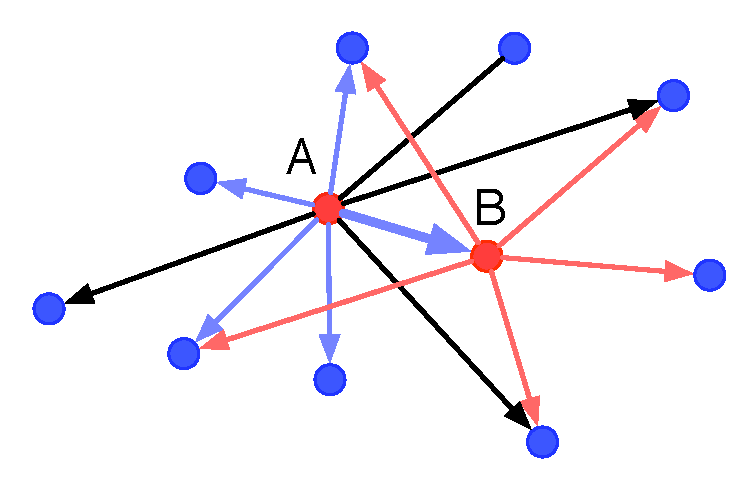
\includegraphics[width=.8\linewidth]{figures/rbf_stencils.pdf}
  \caption{RBFFD Stencils. Each node of the stencil is connected to
    $n_z-1$ stencil nodes in addition to itself. In the figure, node
    $A$ is connected to $B$, but $B$ is {\em not\/} connected to
    $A$. Thus adjacency graph of $A$ is not-symmetric.}
  \label{fig:rbf_stencils}
\end{figure}

Many problems in fluid dynamics and in the geosciences require the
solution to transport equations of the form
\begin{equation}
\pf{Q}{t} = f(Q,\grad{Q},\Laplacian{Q})  \label{eq:Q}
\end{equation}
where $Q$ is a vector of unknowns.
For example, in solving a system of equations, it is
often necessary to compute the derivative of multiple functions along
the same coordinate direction,
typically four for the Euler equations, or five for the Navier-Stokes
equations. Multiple right-hand sides transform a SpMV into a SpMM
(Sparse Matrix/dense Matrix multiplication), which improves register
utilization and decreases cache misses by vectorizing over the
multiple source vectors. Further improvements are possible by
recognizing that different derivative matrices (e.g., gradient and 
Laplacian operators), 
have the same sparsity distribution as long as the derivative stencils
remain unchanged; only the values in the sparse matrix vary. 
Thus, rather than computing a derivative of multiple
functions, one can calculate multiple derivatives of a single
function. The increased memory bandwidth due to an increase in the
number of derivative matrices is offset by better cache utilization,
leading to an overall performance benefit. In practice however, the number of 
vectors whose derivatives are required is limited, capping the 
performance of the matrix/vector multiplication. Similarly, the number
of different derivatives in a particular computation is finite. It is 
for this reason that we seek to combine the benefits of multiple
vectors and multiple matrices simultaneously. We limit this initial 
study to four vectors and four matrices. 

In discrete form, Equation (\ref{eq:Q}) becomes
$$
  y^{i,j} = A^i x^j 
$$ where $j$ ranges over the number of source vectors, $i$ ranges of
  the number of derivative matrices and there are $i*j$ output vectors
  $y$ (graphically shown in Figure~\ref{fig:struct_comp}).

\begin{figure}
  \centering

  \[ \left( \begin{array}{cccc}
    y^{1,1} & y^{1,2} & y^{1,3} & y^{1,4} \\
    y^{2,1} & y^{2,2} & y^{2,3} & y^{2,4} \\
    y^{3,1} & y^{3,2} & y^{3,3} & y^{3,4} \\
    y^{4,1} & y^{4,2} & y^{4,3} & y^{4,4} 
  \end{array} \right)
  = \left(
  \begin{array}{c}
    A^1\\
    A^2\\
    A^3\\
    A^4
  \end{array}\right)
  \times \left(x^1 x^2 x^3 x^4 \right) \] 
  
  \caption{Structure of the computation.}
  \label{fig:struct_comp}
\end{figure}


